% TODO for a $16\times 16$ segmentation patch there exist, in theory $2^256$ possible edge masks. Due to the inherent structure in image patches however, not all of them are likely, and those containing simple structures are prevalent.
% TODO put an image of decision of 4 trees in one pixel
\chapter{Capturing image edge structure} %Structured random decision forests}
\label{Chapter2}
\settocdepth{subsection}
In this chapter we discuss the recent edge detection works by Doll\'ar and Zitnick~\cite{DollarICCV13edges,Dollar2015PAMI}. Their algorithm - Structured edge (SE) takes a data-driven approach to learning of semantic edges. % Let the data speak for itself
%Their goal is
They manage to achieve accurate and fast edge detection. % real-time

By ``structure'' in image edges % as well as in SF leaves
we mean the fact that local image patches are known~\cite{Ren2006figure,LimZD13} to show % exhibit
notable %prominent
forms of local structure (some examples in \fref{fig:srf-structure-in-edge-patches}). As edges are interdependent, often shapes like straight and curved lines, T-junctions and Y-junctions, convexities, sharp corners and parallel lines are to be observed in a local neighbourhood.

\textbf{Capturing more context:} A family of learning approaches have tried to leverage local context to organise images - discover image edges, or recognise %discern
figure from background objects. First the Boosted Edge Learning (BEL) algorithm~\cite{dollar2006supervised} made at each location in the image an independent binary decision as to the presence or absence of image edge. Noticing the abundance of edge structure in a local patch, \textit{sketch tokens}~\cite{LimZD13} and \textit{shapemes}~\cite{Ren2006figure} organise local edge shapes by clustering. 
The Structured forest (SF)~\cite{DollarICCV13edges} takes this idea a step further and keeps all local segmentation patches it has seen at training time in the leaves of its decision trees. By abstaining from using pre-defined classes of edge patches, clustering, or averaging \textbf{to model local edge context}, the SF framework has the potential to learn subtle variations in edge structure. It is flexible - it is able to adapt to the training dataset at hand by letting the data speak for itself. That is one of the reasons for its highly accurate edge detection.

\textbf{Structured forest ``knows'' image edge context:} Precisely the ability of the structured forest to predict a local segmentation mask given an input image patch is so important to us. Even better, the edge detector SE could provide as a by-product the segmentation predictions that it has made at every image location. We would like to use this information in order to obtain image segmentation.

In this chapter we review the SE edge detector and elucidate why it is a good first-step choice for our task of semantic segmentation.

\section{Structured forests}
\settocdepth{section} % avoid listing this in the toc, but give it a number in the text
\subsection{Random decision forests}
\settocdepth{subsection}
Random forest (RF) is a recently introduced~\cite{Breiman01} learning approach which has found applications in computer vision~\cite{KontschiederBBP11,LimZD13,DollarICCV13edges,Dollar2015PAMI} due to its speed both at training and testing time, high accuracy, and robustness to noise.

A random decision forest is a collection %an ensemble %a combination 
of tree predictors - classifiers or regressors~\cite{breiman1984classification}. Here ``tree'' is used in the computer science sense to denote an abstract data structure (ADS) - a graph without cycles. 
The predictive power of the forest depends on the strength of the individual trees and their de-correlation. Therefore every tree is constructed based on a vector, sampled independently and randomly from the space of possible vectors. The randomness could be \wrt the training examples that are made available to each tree and\slash or the set of features that are being considered at each node of a decision tree.

Criminisi \etal~\cite{Criminisi12} provide a survey of decision tree methods.

Nowozin~\cite{Nowozin12improvedinformation,nowozin2014decision} discusses bias in the estimation of information gain for making split decisions at each node during decision tree training. He proposes estimators which lead to training better trees, yielding improved predictive performance.

\subsubsection{Structured learning}
By definition, {\it structured learning} means that the input and output spaces can be arbitrarily complex. Examples are images, graphs, strings, bounding boxes, joints positions for object pose estimation, folds of proteins, sequences of actions. The initial methods proposed for the task of structured learning were probabilistic graphical models (PGMs) and structured support vector machines (structured SVMs).

Kontschieder \etal~\cite{KontschiederBBP11} were first to observe that RFs are applicable to the problem of structured learning. They remark that any type of input could be given to RF and they could preserve %conserve 
any type of output in the leaves of the trees. They extend the RF framework to work with structured class labels and use it to perform semantic image labelling (\textit{bike, cow, car, building, road \etc}).

\section{Structured edge algorithm outline}
The key to edge detection using SF is that the decision for a single point is made based on an image patch centred at it. A large enough patch contains low-level features as well as mid-level context information (see \fref{fig:srf-structure-in-edge-patches}).

\begin{figure}[ht!]
\centering
 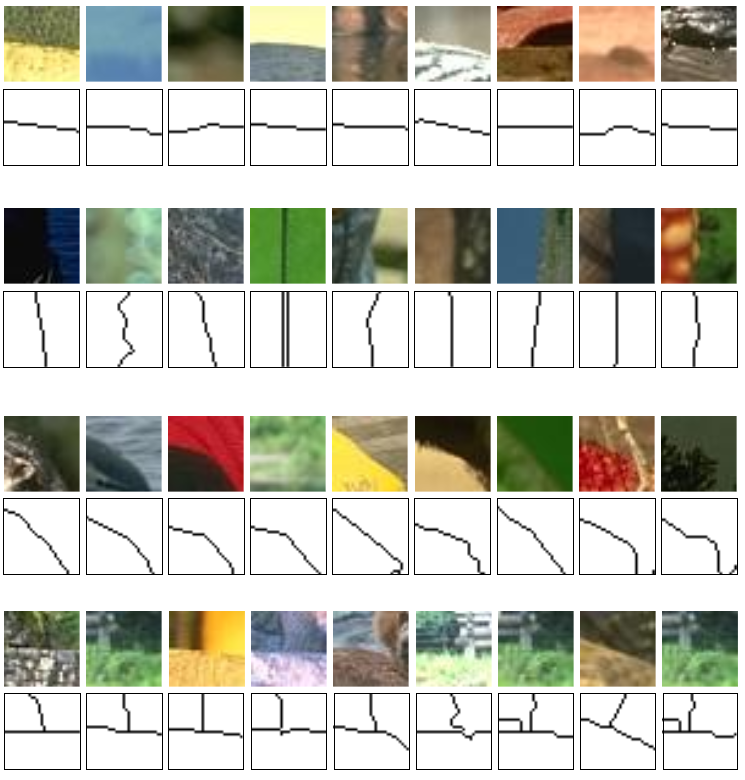
\includegraphics[width=0.5\textwidth]{images/srf/structure-in-edge-patches.png}
\caption{Local edge patches exhibit similar structure. Image patches and the human-%hand-
drawn edges present in them. Cropped from BSDS500, courtesy of~\cite{DollarICCV13PresentationSlides}.}
\label{fig:srf-structure-in-edge-patches}
\end{figure}

SE is an example of supervised machine learning. During training time it is presented with patches and their ground truth annotations (local segmentations). It learns parameters that enable it to make predictions at testing time as to the most likely segmentation of fresh, unseen so far patches. For edge detection, it agglomerates those multiple patch decisions to obtain a probability of boundary (probabilistic edge map) for an entire image.

\section{Training - growing a decision forest}
A RF is trained by recursively growing its decision trees. For the task of edge detection, the training data is a total of 1 million training samples. Half of those are positive examples - a patch containing an edge and its hand-labelled segmentation. The other half are negative examples - so-called ``background patches''. To grow a decision tree means to learn what is a good way of redistributing the input data presented to the tree (at its root node) into its leaves. Such a distribution to the tree leaves would be good if in the end similar training samples are grouped together - in the same decision tree leaf. In the following we discuss binary decision trees, as this is the data structure used in practice by the SE algorithm. It is trivial to extend the algorithm to use general trees by making a multi-class decision at each node. 

% \textbf{Training is redistributing the data towards the leaves of a binary tree:} 
\subsection{Learning the split function}
So at each node a binary decision must be made how to separate the training data into the left and right child sub-trees. Initially the root of the tree contains all training data available to the tree. A split function $h(x,\theta_j)\in\{0,1\}$ determines to which child an input training sample $x$ is forwarded. The parameter $\theta_j$ is what must be learnt for each node $j$ during training. A criterion based on information gain is introduced to decide on optimal %good 
splits. Splitting is done in such a way so as to minimise entropy in the nodes. In this algorithm Gini impurity is used. Some of the improvements proposed by Nowozin~\cite{Nowozin12improvedinformation,nowozin2014decision} regarding entropy estimators are adopted in this work. Growing by splitting a node continues until either 1) a certain maximal tree depth is reached, or 2) sufficient purity of nodes is achieved.

The goal is to cluster in the leaves of the trained structured decision tree segmentation patches that correspond to input features which are as similar as possible. The nett effect is that similar segmentation patches should end up in the same leaf, see \fref{fig:structured-decision-tree-node-split}.

\settocdepth{section}
\subsection{Key contribution of the work}
\settocdepth{subsection}
The ``structured output'' in the case of the SE algorithm is a $d\times d$ segmentation patch (in practice they set $d = 16$). 
As the segmentation patch space is high-dimensional and complex, it is non-trivial to compute information gain in order to split the set of inputs into two subsets.

\textbf{Proxy label space:} They introduce a mapping to a simpler, lower-dimensional discrete space. The information gain computed on it is a sufficient approximation of that of the original output space without being prohibitively expensive to compute. Thus it is possible to compute distance, or, analogously, similarity, between output segmentation. In effect, similar output segmentations are clustered together.

\begin{figure}[ht!]
\centering
 \subfigure[A training sample is a pair of image patch and its corresponding ground-truth segmentation.]{%
  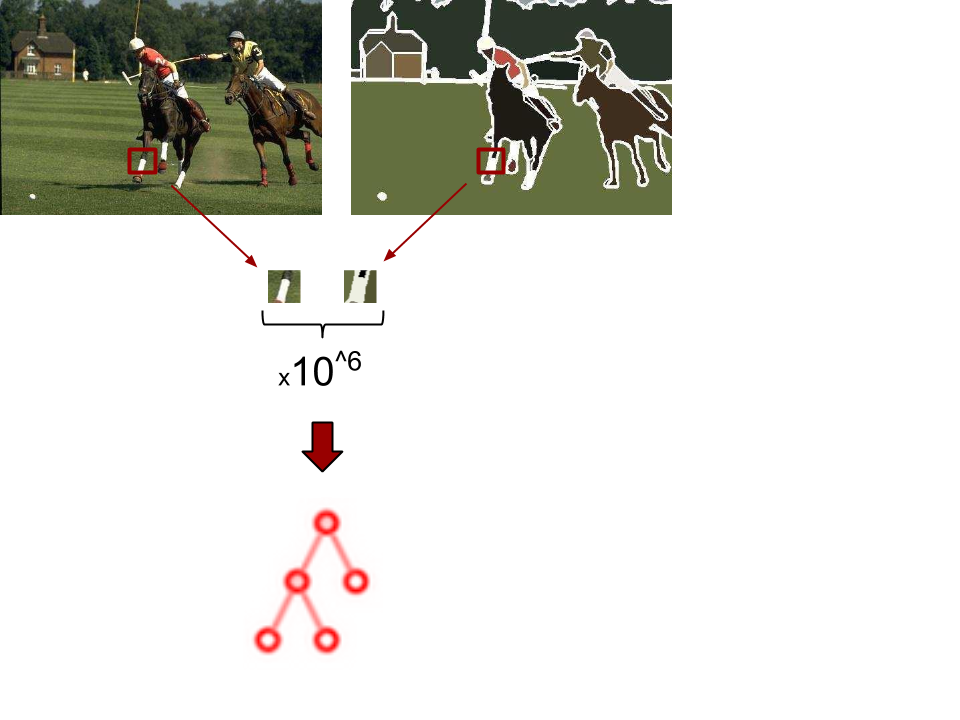
\includegraphics[width=0.5\textwidth]{images/srf/structured-decision-tree-training.png}
 }
 \subfigure[Splitting of training data at a node of a decision tree]{%
  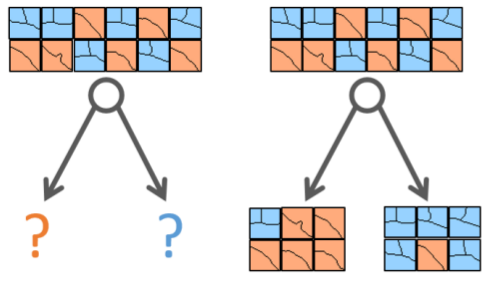
\includegraphics[width=0.3\textwidth]{images/srf/structured-decision-tree-node-split.png}
  \label{fig:structured-decision-tree-node-split}
 }
\caption{Training of a decision tree. \protect\subref{fig:structured-decision-tree-node-split} courtesy of~\cite{DollarICCV13PresentationSlides}.}
\label{fig:srf-training}
\end{figure}

\settocdepth{section}
\subsection{Introducing randomness for diversity of the decision forest}
\settocdepth{subsection}
Part of the accuracy in prediction of the RF framework comes from ensuring sufficient diversity of trees. One way to achieve this, and how it is done in the SE algorithm, is by introducing randomness at each decision node. This is done by subsampling the input features that are taken into account when optimising the split at the tree node. SF achieves robust results by combining the output of $T$ decorrelated trees. Because of the small correlation of the trees in the ensemble, even small forests manage good performance - we later use SE with $T=4$.

\section{Inference}
Unlike other structured learning methods, no optimisation is required to make a prediction. Inference using SF is straightforward. A decision forest is an ensemble of $T$ \textit{independent} trees. To make a prediction, the individual predictions of the trees are combined as prescribed by the ensemble model. Here averaging is performed on the output edge patches.

\subsection{Structured decision tree inference}
The test sample - a feature vector computed based on an input image patch $x$, travels down the tree. Decisions whether it should be routed to the left or right child of a node are made according to the parameters learnt during training. When a leaf node is reached, it contains a set of most likely segmentations, and each of those could be associated with the input $x$.

\textbf{Ensemble model:} In the context of random forests the term ``ensemble model'' defines how to combine multiple predictions into a single prediction. Somewhat confusing, in the paper~\cite{DollarICCV13edges}, this refers to two different things:
\begin{enumerate}
 \item{in decision tree inference:} in order to associate a prediction with the each leaf (like in~\ref{fig:srf-tree-inference}). To this end, the medoid segmentation patch \textit{for the proxy output space} is chosen. This is the one that minimises the sum of distances to all others in the leaf patch, see~\ref{fig:srf-leaf}. The medoid is the only patch that is subsequently used out of all those in the tree leaf. Note that only patches which have been observed during training can be predicted during testing %by the SF
 in this scenario.
 \item{in detection:} to make the final edge detection, a means to combine multiple overlapping decisions is necessary. Details will be given shortly in \textsection~\ref{sec:ch2-edge-detection}.
\end{enumerate}

\begin{figure}[ht!]
\centering
 \subfigure[Image patches used as input, which ended up clustered in the same structured tree leaf.]{%
  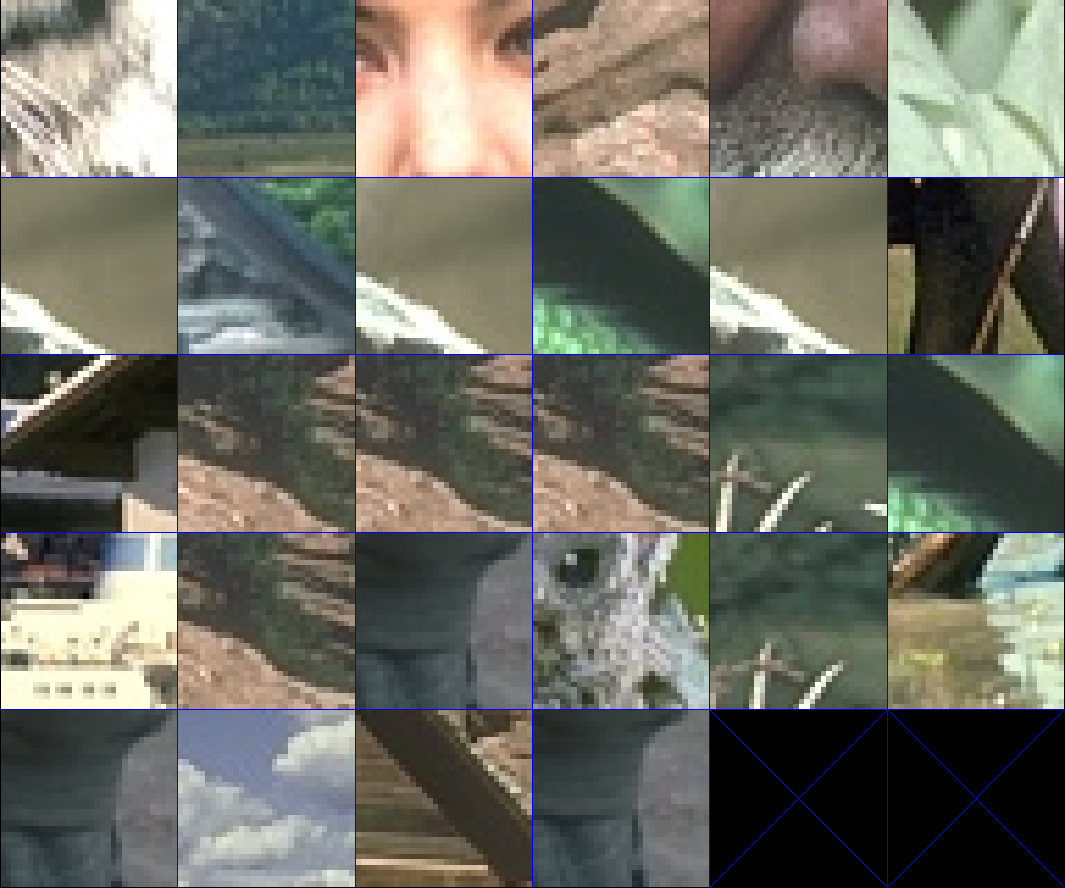
\includegraphics[width=0.45\textwidth]{images/srf/sf-leaf-imgs.png}
  \label{fig:sf-leaf-imgs}
 }
 \subfigure[Corresponding segmentation patches in a structured tree leaf. Upper left is the medoid.]{%
  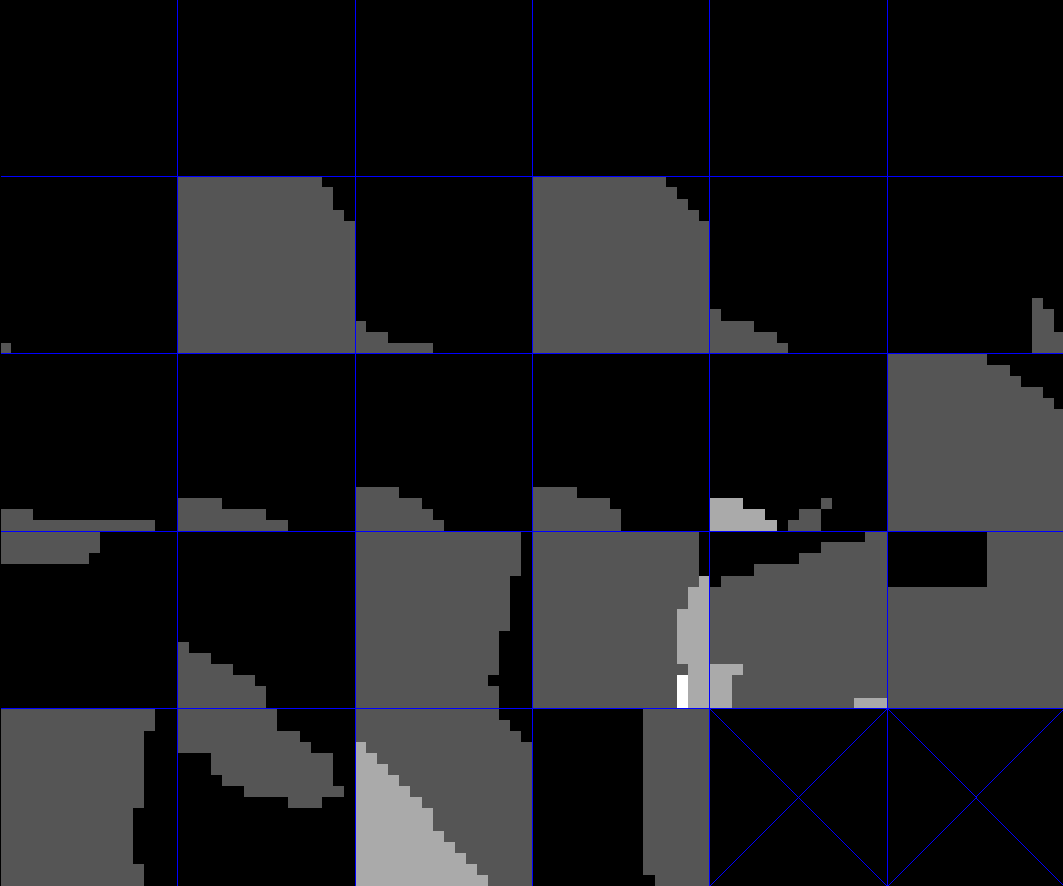
\includegraphics[width=0.45\textwidth]{images/srf/sf-leaf-segs.png}
  \label{fig:sf-leaf-segs}
 }
\caption{Contents of a decision tree leaf. Notice that while the input patches (and consequently, the features computed based on them), are sufficiently similar, the same cannot be said about the segmentation patches. The representative prediction is the medoid - upper left.}
\label{fig:srf-leaf}
\end{figure}

\begin{figure}[ht!]
\centering
 \subfigure[Decision tree inference]{%
  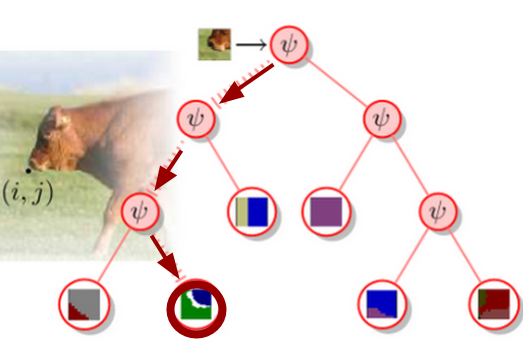
\includegraphics[width=0.57\textwidth]{images/srf/srf-tree-inference.png}
  \label{fig:srf-tree-inference}
 }
 \subfigure[Decision forest as an ensemble of multiple trees]{%
  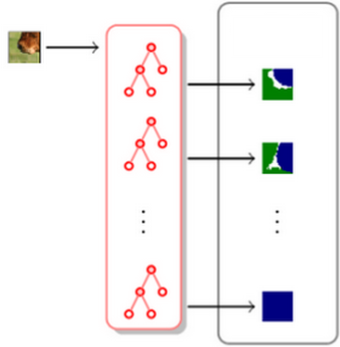
\includegraphics[width=0.4\textwidth]{images/srf/srf-inference-an-ensemble-of-trees.png}
  \label{fig:srf-inference-an-ensemble-of-trees}
 }
\caption{Inference with structured random forest. Images courtesy of~\cite{DollarBlog2013srf}}
\label{fig:srf-inference}
\end{figure}

\subsection{Edge detection}
\label{sec:ch2-edge-detection}
Now that a most-likely segmentation can be obtained given an input image patch, how to do edge detection on a whole image?

\subsubsection{Sliding window}
Structured labels capture information about entire pixel neighbourhood. Therefore a small number - $T$ of tree predictions per pixel suffice for high edge detection quality. Detection is performed by sliding a window across the image, with a stride $s = 2$, and evaluating, in a chequerboard-pattern a set of $T$ trees. So a total of $2T$ trees are trained. Each of the trees makes a prediction for the given location, many are overlapping. For a patch side of $d = 16$, with $T=4$, each pixel receives $\frac{T*d*d}{s*s}=256$ independent decisions.

\subsubsection{Averaging of overlapping decisions}
The individual decisions are local segmentation masks. As discussed in \cref{Chapter1}, it is fairly easy to obtain an edge map, given a segmentation. This is how the multiple patches decisions have to be represented in order to aggregate the information in them for the purposes of edge detection. The combining is done by superimposing, %merging
and then averaging the edge maps from multiple overlapping patches. %decisions. 
This is referred to in the paper~\cite{DollarICCV13edges} as ``custom ensemble model''.

\section{Discussion}
At the time it was published, SE algorithm showed state-of-the-art performance on the now standard benchmark for the task of boundary detection - BPR on BSDS500~\cite{Arbelaez11}. The algorithm is tested on other datasets and the models learnt are capable of successfully finding edges in images from datasets that they were not specifically trained for. This is reassuring - it means that the detector is able to generalise - its knowledge is universal, instead of overly adapted to %fit for 
the contents of a specific dataset.

\settocdepth{section}
\subsection{Alternative way of capturing context}
A different approach is taken by Hallman and Fowlkes in their \textbf{Oriented edge forests (OEF)} paper~\cite{Hallman2014} which was published towards the end of the current research work. They use a decision forest classifier to learn to distinguish between straight-line edges of different position and orientation within an image patch, see \fref{fig:OEF-oriented-patch-space}. Although they use a set of pre-defined edge classes, local sharpening of the edges helps them capture fine variations in edge shape. They currently (Feb 2015) achieve best results on the BSDS500 benchmark.

\begin{figure}[ht!]
\centering
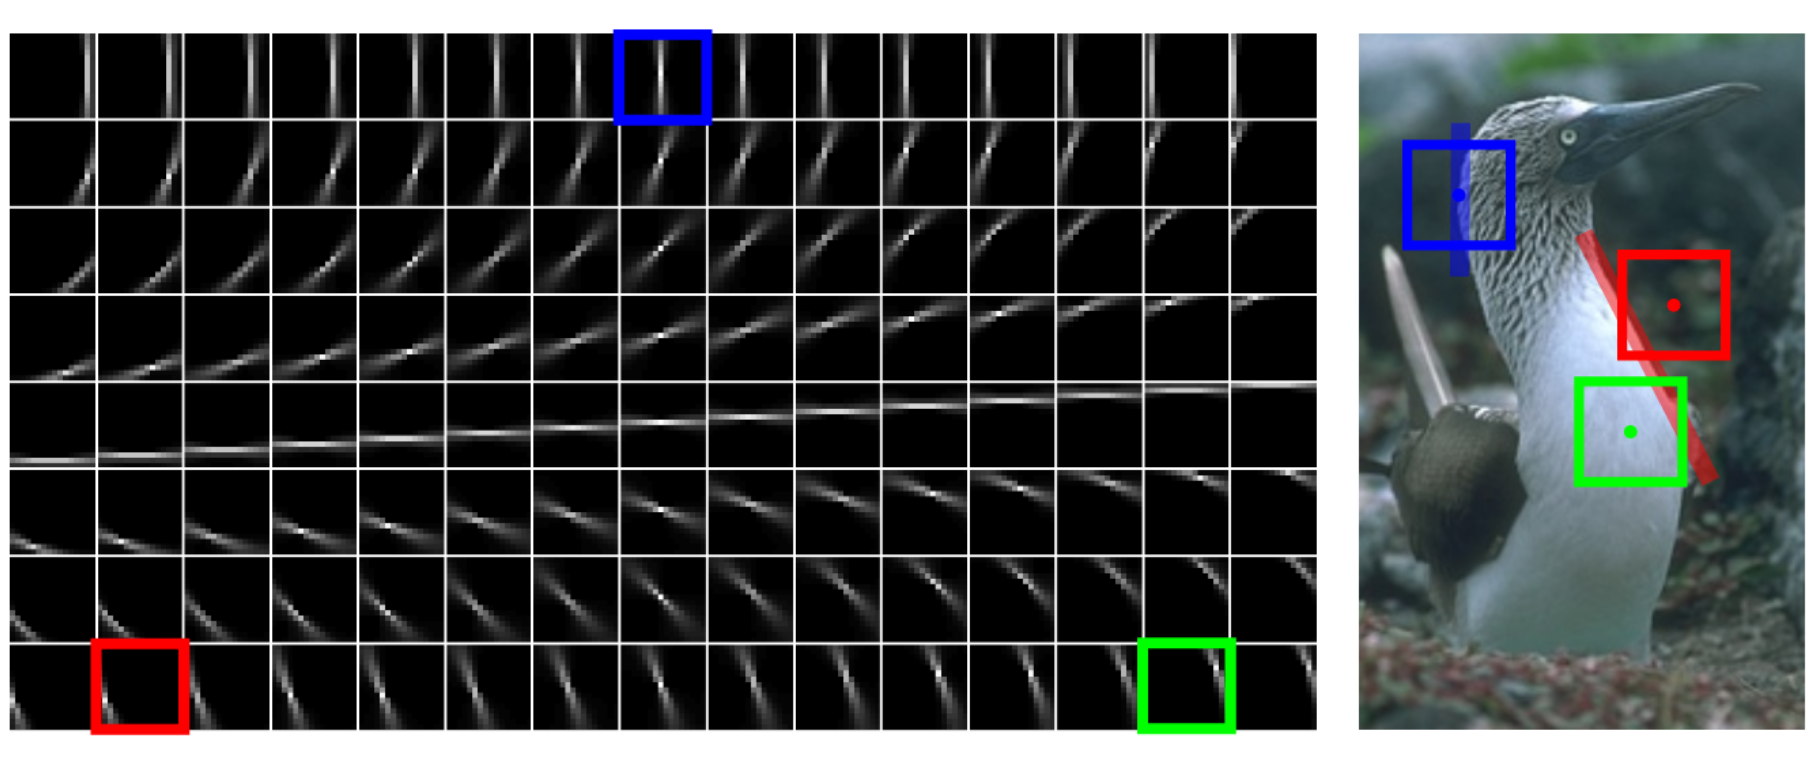
\includegraphics[width=0.8\textwidth]{images/OEF-oriented-patch-space.png} % not in srf/ subfolder as it is more ``related work''
\caption{Decision forest predicts a probability distribution over a fixed patch space (given on the left). Images courtesy of~\cite{Hallman2014}}
\label{fig:OEF-oriented-patch-space}
\end{figure}

\textbf{OEF for image segmentation:} The output of their algorithm is an oriented probability of boundary $E(x,y,\theta)$. Therefore, it would be a natural fit for the OWT-UCM pipeline described in~\cite{Arbelaez11}. The resulting procedure, which they title ``OEF-OWT-UCM'' allows to use the edge detection results to obtain a hierarchical image segmentation. They report, however, misalignments due to quantisation mismatch of the orientation angles between their algorithm and gPb-OWT-UCM of~\cite{Arbelaez11}.

\subsection{Strong points of SE}

\begin{itemize}
 \item accurate edge detector,
 \item fast at training time (which is done offline),
 \item real-time speed at test time - during edge detection,
 \item has potential as a general-purpose edge detector, %TODO add note - gPb seems to be highly-tuned for the BSDS500 dataset
 \item is able to predict a most-likely segmentation for a given input patch,
 \item can be augmented to store all those intermediate predictions made during the edge detection.
\end{itemize}

